\chapter{Complexidade Computacional}

% Funções de complexidade, que satisfazem aos axiomas de Blum
\newcommand{\PhiDT}{{\mathcal{T}}} % Tempo determinístico
\newcommand{\PhiDS}{{\mathcal{S}}} % Espaço determinístico
\newcommand{\PhiNT}{{\mathcal{N\!T}}} % Tempo não-determinístico
\newcommand{\PhiNS}{{\mathcal{N\!S}}} % Espaço não-determinístico

\emph{Complexidade} é a quantidade de recursos
que uma máquina de Turing gasta
para computar determinada função
ou para decidir pertinência a uma linguagem
\cite[p.~285]{HopcroftUllman1979}.
Os recursos mais importantes para a teoria de complexidade computacional
são o espaço e o tempo,
em máquinas de Turing determinísticas e não"=determinísticas.

Embora seja possível trabalhar com estas medidas diretamente,
muitos resultados para uma medida
possuem análogos em outra medida.
Começaremos,
na seção~\ref{axiomas_blum},
com uma discussão sobre a teoria de complexidade computacional axiomática,
e definiremos as medidas de complexidade padrão na seção~\ref{medidas_padrao}.

\section{Teoria de Complexidade Axiomática: Axiomas de Blum}
\label{sec:blum_axioms}

\begin{definition}
    Seja $\phi$ uma enumeração de Gödel aceitável.
    Uma \emph{medida de complexidade} é uma função
    $\Phi: \{0, 1\}^* \times \{0, 1\}^* \to \mathbb N$,
    que satisfaz aos seguintes axiomas:\footnotemark
    \begin{enumerate} [label=\textbf{Axioma \arabic*}, ref=\arabic*, align=left]
        \item
            \label{ax:blum_def}
            $\Phi(x, y)$ está definido
            se, e somente se,
            $\phi_x(y)$ está definido.
        \item
            \label{ax:blum_rec}
            A função $R(x, y, m)$,
            definida como $1$ se $\Phi(x, y) = m$,
            e $0$ caso contrário,
            é recursiva total.
    \end{enumerate}

    \footnotetext{
        A definição original de \citeonline[p.~3]{Blum1967}
        é dada no contexto do cálculo de funções de inteiros.
        Em particular,
        as enumerações de Gödel aceitáveis são indexadas por números,
        não por cadeias de $\{0, 1\}^*$.
        Esta adaptação é baseada na definição de \citeonline[p.~156]{Papadimitriou1994}.
    }
\end{definition}

O axioma~\ref{ax:blum_rec}
nos dá um semialgoritmo para calcular $\Phi(M, x)$.
Entretanto, pelo axioma~\ref{ax:blum_def},
não podemos ir muito além disso,
pois $M(x)$ não está definido para todo $M$ e $x$.
De fato, sequer podemos decidir se $\Phi(M, x)$ existe.

\begin{example}
    \label{ex:time_complexity}
    \simbolo{$\PhiDT$}{Complexidade de Tempo}
    A \emph{complexidade de tempo},
    que denotaremos por $\PhiDT$,
    é a função que diz quantos movimentos
    uma máquina de Turing faz até retornar uma resposta.
    Isto é,
    \begin{equation*}
        \PhiDT(M, x) = \begin{cases}
            k, & \text{
                \parbox{0.6\textwidth}{
                    se $M$ executa exatamente $k$ passos em $x$ antes de parar.
                }
            } \\
            \text{indefinido}, & \text{
                \parbox{0.6\textwidth}{
                    caso $M$ nunca pare de computar $x$.
                }
            }
        \end{cases}
    \end{equation*}
    Para determinar se $\PhiDT(M, x) = k$,
    execute a máquina $M$ por $k$ passos
    e veja se é a primeira vez que
    $M$ atinge um estado aceitador.
    E, como $\PhiDT(M, x)$ só está definido se $M$ para ao computar $x$,
    $\PhiDT$ satisfaz aos dois axiomas de Blum.
\end{example}

\begin{example}
    \label{ex:space_complexity}
    \simbolo{$\PhiDS$}{Complexidade de Espaço}
    Para a \emph{complexidade de espaço},
    que denotaremos por $\PhiDS$,
    assumiremos que $M$ possui uma fita somente"=leitura
    específica para a entrada.
    \begin{equation*}
        \PhiDS(M, x) = \begin{cases}
            k, & \text{
                \parbox{0.6\textwidth}{
                    se~$M$ para ao computar~$x$,
                    tendo lido exatamente~$k$ células
                    de uma de suas fitas de trabalho
                    e no máximo $k$~células nas demais fitas.
                }
            } \\
            \text{indefinido}, & \text{
                \parbox{0.6\textwidth}{
                    se $M$ nunca parar ao computar $x$.
                }
            }
        \end{cases}
    \end{equation*}
    Precisamos desta definição intrincada
    pois~$M$ pode não ler $k$~células de todas as suas fitas,
    apenas de algumas.

    Claramente o axioma~\ref{ax:blum_def} é satisfeito.
    Para o axioma~\ref{ax:blum_rec},
    o algoritmo é um pouco mais complicado.

    Comece executando $M$ em $x$.
    Caso $M$ extrapole $k$ células lidas
    em alguma de suas fitas,
    podemos rejeitar a entrada
    (isto é, $\Phi(M, x) = k$ é falso).
    Caso contrário,
    existirá um número finito de configurações da máquina.

    Existem~$|\Gamma|^k$ possíveis fitas com $k$ termos
    e $k+1$ possíveis posições da cabeça de leitura;
    teremos, portanto,
    $(k+1)|\Gamma|^k$~diferentes configurações para cada fita.
    Para $l$ diferentes fitas e $|Q|$~possíveis estados da máquina,
    existem, no máximo,
    \begin{equation}
        |Q| \left((k+1)|\Gamma|^k\right)^l
        \label{eq:configurations_count}
    \end{equation}
    possíveis configurações.
    Portanto, se a máquina executar
    mais movimentos do que este número,
    significa que ela entrou em loop.
    Podemos rejeitar a entrada.%
    \footnote{
        Este cuidado adicional é imprescindível
        para garantir que o predicado
        ``$\Phi(M, x) = k$''
        seja decidível,
        não apenas semidecidível.

        Note que precisamos rejeitar a entrada
        caso a máquina entre em loop
        porque $\Phi(M, x)$ só está definido
        quando $M(x)$ está
        --- não é o caso se $M$ entra em loop
        ao computar $x$.
    }

    E, por último,
    caso $M$ pare,
    precisamos nos assegurar que,
    de fato,
    em alguma das fitas $k$ células foram lidas.
\end{example}

\begin{example}
    \label{ex:nondeterministic_complexity}
    \simbolo{$\PhiNT$}{Complexidade de Tempo não"=determinística}
    \simbolo{$\PhiNS$}{Complexidade de Espaço não"=determinística}
    Podemos adaptar $\PhiDT$ e $\PhiDS$
    para máquinas de Turing não"=determinísticas.%
    \footnote{
        Tecnicamente,
        as denominações usuais,
        ``complexidade de tempo/espaço não"=determinística''
        ou ``tempo/espaço não"=determinístico''
        estão erradas;
        não é o tempo ou espaço ou a complexidade que são não"=determinísticos,
        mas sim o modelo de máquina ao qual nos referimos.

        Entretanto, toleraremos este abuso de nomenclatura neste texto.
    }

    A complexidade de tempo não"=determinística,
    que denotaremos por $\PhiNT(M, x)$,
    definiremos como sendo a maior quantidade de movimentos
    tomadas por $M$ ao computar $x$
    dentre todas as escolhas de transições possíveis.

    Analogamente,
    definiremos a complexidade de espaço não"=determinística,
    que denotaremos por $\PhiNS(M, x)$,
    como sendo a maior quantidade de células lidas
    em qualquer dos ramos da computação de $M$ em $x$.
    Aqui, precisamos tomar o mesmo cuidado que tomamos
    com $\PhiDS$ para demonstrar o axioma~\ref{ax:blum_rec}.
\end{example}

Observe que, neste exemplo,
jogamos o problema de
explicar como uma máquina não"=determinística computa uma função
para ``debaixo do tapete''.
Voltaremos a este problema no capítulo~\ref{ch:nondeterministic_functions}.
Por ora,
será suficiente nos restringirmos às funções booleanas,
usando a mesma definição usada para decisores.

\begin{example}
    Escolher $\Phi(M, x) = 0$ para todo $M$ e $x$
    satisfaz ao axioma~\ref{ax:blum_rec},
    mas não ao axioma~\ref{ax:blum_def},
    pois $\Phi(M, x)$ está definida mesmo quando $M(x)$ não está.
    Já definir $\Phi(M, x) = |M(x)|$
    satisfaz ao axioma~\ref{ax:blum_def},
    mas não ao axioma~\ref{ax:blum_rec},
    pois poderíamos resolver o problema da parada:
    dada uma máquina $M$, podemos modificá"=la
    para apagar sua fita logo antes de parar.
    Então, para esta $M'$,
    $\Phi(M', x) = 0$ se, e somente se,
    a $M$ original para ao computar $x$.
    Estes dois exemplos mostram que os axiomas são independentes
    \cite[p.~3]{Blum1967}.
\end{example}

Podemos ver que as medidas $\PhiDT$ e $\PhiDS$ estão relacionadas.
Para ler uma posição da fita,
é necessário gastar ao menos uma unidade de tempo.
Ou seja,
\begin{equation*}
    \PhiDS(M, x) \leq \PhiDT(M, x).
\end{equation*}
E, de acordo com o raciocínio do exemplo~\ref{ex:space_complexity},
para todo $M$ existe algum $c$ que
\begin{equation*}
    \PhiDT(M, x) \leq c^{\PhiDS(M, x)}.
\end{equation*}
De fato, podemos relacionar quaisquer duas medidas de complexidade.

\begin{theorem}
    \label{thm:measure_related}
    Dadas duas medidas de complexidade $\Phi$ e $\hat \Phi$,
    existe uma função recursiva $r$ tal que
    \begin{equation*}
        \Phi(M, x) \leq r( x, \hat \Phi(M, x))
    \end{equation*}
    para todo $M$ e quase todo $x$.%
    \footnote{
        Um predicado é ``verdadeiro para quase todo $n$''
        quando ele é falso para apenas uma quantidade finita de números $n$.
        Equivalentemente,
        é quando existe algum $n_0$ tal que
        o predicado é válido para todo $n > n_0$.
    }
\end{theorem}

\begin{proof}
    Defina
    \begin{equation*}
        r( x, k ) = \max \{ \Phi(M, x) \mid
            \text{A descrição de $M$ é mais curta que $|x|$}
            \text{ e }
            \hat \Phi(M, x) = k
        \}
    \end{equation*}
    Fixado $x$, existe um número finito de máquinas de Turing
    cuja descrição é menor que $|x|$.
    O conjunto na definição acima é um subconjunto desta lista.
    O predicado $\hat \Phi(M, x) = k$ é recursivo.
    Quando este predicado é verdadeiro,
    $M(x)$ está definido, pelo axioma~\ref{ax:blum_def},
    portanto $\Phi(M, x)$ também está definido.
    Concluímos que $r$ é recursiva.

    Agora, para todos os $x$ que são mais longos que a descrição de $M$,
    $\Phi(M, x)$ será um dos elementos do conjunto acima
    para $r( x, \hat \Phi(M, x))$,
    portanto é menor ou igual a este número.
\end{proof}

\citeonline[p.~4]{Blum1967} demonstra uma versão ligeiramente mais forte
deste teorema.
Ele prova que $r$ pode ser tal que,
simultaneamente,
\begin{equation*}
    \Phi(M, x) \leq r( x, \hat \Phi(M, x))
\end{equation*}
e
\begin{equation*}
    \hat \Phi(M, x) \leq r( x, \Phi(M, x))
\end{equation*}
Podemos construir uma função dessas
pegando o máximo de duas funções obtidas
usando o teorema~\ref{thm:measure_related}.

O teorema,
assim como provamos,
não pode ser fortalecido
para que $r$ seja uma função de apenas uma variável.
Considere $A$ uma máquina de Turing
que opere como um autômato finito.
$\PhiDT(A, x) = |x|$ para toda palavra $x$,
enquanto que $\PhiDS(A, x) = 1$ para toda palavra $x$.%
\footnote{
    A complexidade de espaço não é $0$
    pois $A$ é obrigada a ler
    ao menos a célula inicial da sua fita de trabalho,
    embora a máquina não use aquela célula.
}
Se $r$ pudesse depender apenas da segunda variável,
isto é, $r(x, m) = r'(m)$ para alguma função $r'$,
teríamos
\begin{align*}
    |x| &= \PhiDT(A, x) \\
        &\leq r(x, \PhiDS(A, x)) \\
        &= r(x, 1) \\
        &= r'(1)
\end{align*}
que é falso para todo $x$ suficientemente comprido.

Caso $r$ pudesse depender apenas da primeira variável,
isto é, $r(x, m) = r''(x)$ para alguma função $r''$,
teríamos, para todas as máquinas de Turing,
\begin{equation*}
    \PhiDT(M, x) \leq r''(x).
\end{equation*}
Mas, como $r''$ é recursiva
(pois $r$ o é),
podemos construir uma máquina que calcula $r''(x)$,
desperdiça $r''(x)$ movimentos,
e aceita a entrada.
Para esta $M'$,
\begin{equation*}
    \PhiDT(M', x) > r''(x),
\end{equation*}
contradizendo a equação anterior.

No parágrafo anterior,
construímos uma máquina de Turing
que deliberadamente desperdiça tempo
ao computar determinada função.
\citeonline[p.~4]{Blum1967} demonstrou que
é sempre possível desperdiçar recursos computacionais,
quaisquer que sejam estes recursos.
Precisamos de um lema,
vindo direto da teoria das funções recursivas.

\begin{lemma}[Teorema da Recursão]
    Denote por $M_x$ a máquina de Turing
    representada pela palavra $x$.

    Para qualquer função recursiva total $\sigma$,
    existe um valor $m$ tal que
    \begin{equation*}
        M_m(x) = M_{\sigma(m)}(x)
    \end{equation*}
    para todo $x$.
    (Tal valor é chamado de \emph{ponto fixo} para $\sigma$.)
    \label{thm:recursion}
\end{lemma}

\begin{proof}
    Primeiro, construiremos uma máquina $N$ que,
    ao receber $x$ na entrada,
    devolverá um índice\footnotemark{} para $M_x(x)$.
    Isto é,
    para todo $y$,
    \begin{equation}
        M_{N(x)}(y) = M_{M_x(x)}(y),
        \label{eq:diagonal_N}
    \end{equation}
    sempre que $M_x(x)$ existir.
    \footnotetext{
        Um \emph{índice} para uma função recursivamente enumerável $f$
        é um número $i$ que representa uma máquina de Turing para $f$;
        isto é,
        $M_i(x)$ está definido se, e só se, $f(x)$ está definido,
        e, neste caso,
        $M_i(x) = f(x)$
        \cite[p.~130]{EpsteinCarnielli2008}.
    }

    A abordagem direta
    (fazer $M_x$ computar $x$)
    não funciona,
    pois $M_x$ pode nunca parar.

    Observe que não precisamos retornar $M_x(x)$,
    e sim, apenas uma máquina equivalente a $M_x(x)$,
    caso $M_x(x)$ exista.
    Na entrada $x$, $N$ retornará uma máquina que,
    ao receber $y$ na entrada,
    compute $M_x(x)$,
    e, somente após $M_x$ retornar,
    rode $M_x(x)$ em $y$
    (usando uma máquina de Turing universal).

    É importante notar que $N$ sempre pára;
    $M_x(x)$ pode não parar ao computar $x$,
    mas isso significa, apenas,
    que $N(x)$ nunca parará ao computar qualquer coisa
    --- o valor $N(x)$ existirá.

    De posse da máquina $N$, podemos prosseguir.
    Escolha $k$ como sendo um índice para $\sigma \circ N$.
    Isto é,
    \begin{equation}
        M_k(x) = \sigma(N(x))
        \label{eq:k_sigma_N}
    \end{equation}
    para todo $x$.
    Afirmamos que $m = N(k)$
    satisfaz às exigências do teorema.

    De fato,
    \begin{align*}
        M_m(x) &= M_{N(k)}(x) \\
               &= M_{M_k(k)}(x) && \text{Pela equação~\ref{eq:diagonal_N}}\\
               &= M_{\sigma(N(k))}(x) && \text{Pela equação~\ref{eq:k_sigma_N}}\\
               &= M_{\sigma(m)}(x) && \text{Pela definição de $m$.}
    \end{align*}
\end{proof}

\begin{proposition}
    Sejam $f$ e $g$ duas funções recursivas totais,
    e $\Phi$ uma medida de complexidade.
    Então existe uma máquina de Turing $M$ que computa $f$
    tal que
    \begin{equation*}
        \Phi(M, x) > g(|x|)
    \end{equation*}
    para todo $x$.
    \label{thm:resource_waste}
\end{proposition}

\begin{proof}
    Defina a função $h$, de duas variáveis, por
    \begin{equation*}
        h(m, x) = \begin{cases}
            M_m(x) a & \text{se $\Phi(M_m, x) \leq g(|x|)$} \\
            f(x) & \text{caso contrário.}
        \end{cases}
    \end{equation*}
    ($M_m(x)a$ é o valor de $M_m(x)$ concatenado com a letra $a$.)

    Observe que $h$ é uma função computável,
    pois $\Phi$, $g$ e $f$ o são,
    e, caso $\Phi(M_m, x)$ esteja definido,
    $M_m(x)$ também estará.

    Construa a função $\sigma$ que,
    ao receber $m$ na entrada,
    altere"=a para que,
    quando ela receber $x$ na entrada,
    compute $h(m, x)$.
    Ou seja,
    \begin{equation*}
        M_{\sigma(m)}(x) = h(m, x).
    \end{equation*}
    $\sigma$ pode, por exemplo,
    codificar $m$ nos estados de $\sigma(m)$;
    esta máquina imprimirá $m$ na fita,
    ao lado do $x$,
    e executar uma sub"=rotina que computa $h$ no restante.

    Pelo teorema da recursão (lema~\ref{thm:recursion}),
    $\sigma$ possui um ponto fixo $m_0$.
    Demonstraremos que $m_0$ satisfaz às exigências do teorema.

    Caso a função $h$, ao computar o valor de $h(m_0, x)$
    para algum $x$,
    tenha escolhido a primeira cláusula,
    a saída final de $\sigma(m_0)$ teria sido
    $M_{m_0} (x)$ concatenado com $a$,
    que é diferente de apenas $M_{m_0}(x)$.
    Portanto, $m_0$ não seria um ponto fixo de $\sigma$,
    contradizendo o teorema da recursão.

    Portanto, $h$ nunca seleciona a primeira cláusula
    ao computar $h(m_0, x)$, para qualquer $x$.
    Isto significa que $\Phi(m_0, x) > g(|x|)$ para todo $x$,
    o que garante a exigência de complexidade,
    e que
    \begin{equation*}
        M_{\sigma(m_0)}(x) = f(x).
    \end{equation*}
    Mas, como $m_0$ é um ponto fixo de $\sigma$,
    a própria $m_0$ já computava $f$ antes de passar por $\sigma$,
    o que prova a exigência da função.
\end{proof}

Em outras palavras,
código ruim pode ser feito em qualquer linguagem.

\subsection{Classes de Complexidade}

\begin{definition}
    Dada uma medida de complexidade $\Phi$
    e uma função recursiva total
    $f: \mathbb N \rightarrow \mathbb N$,
    a \emph{classe de complexidade $f$} com relação a $\Phi$
    é o conjunto
    \begin{equation*}
        \mathcal C_\Phi(f) = \{ L(M) \mid \Phi(M, x) \leq f(|x|)
            \text{ para quase todos os $x$}
        \}.
    \end{equation*}
\end{definition}
Permitiremos que a complexidade de $M$
possa ser maior que $f$ para um número finito de elementos
para simplificar as demonstrações.

Embora faça sentido definir $\mathcal C_\Phi(f)$
para funções $f$ arbitrárias,
a exigência de $f$ ser recursiva total
torna as classes de complexidade
sucetíveis a argumentos por diagonalização.

Por exemplo,
podemos mostrar que
nenhuma classe de complexidade contém todas as linguagens recursivas.
Precisamos de um lema.

\begin{lemma}
    Existe um mapeamento bijetivo computável
    entre $\mathbb N$ e $\mathbb N \times \mathbb N$.
\end{lemma}

\begin{proof}
    Percorra o caminho descrito pelas setas na figura~\ref{passeio_cantor}.

    \begin{figure}[h]
        \centering
        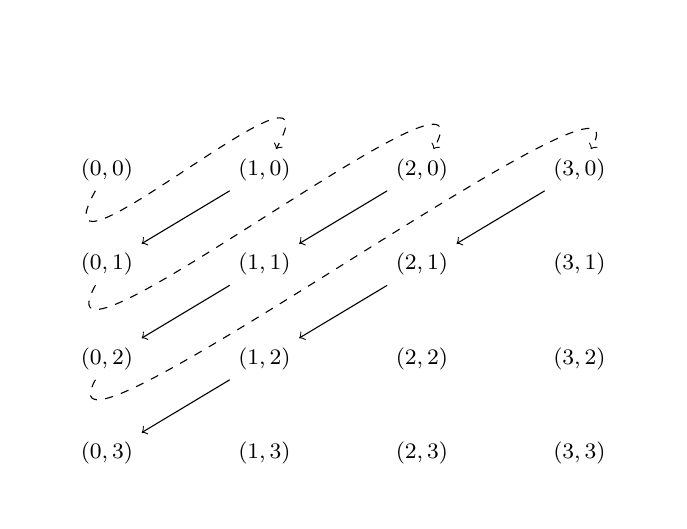
\begin{tikzpicture}
            \foreach \i in {0,...,3}
            \foreach \j in {0,...,3} {
                \node[font=\footnotesize]
                    (a\i\j) at (2*\i, -1.2*\j) {$(\i, \j)$};
            }

            \foreach \a/\b in {a00/a10, a01/a20, a02/a30} {
                \draw[->, dashed] (\a) .. controls
                +(-1,-1.8) and
                +(1, 1.8) .. (\b);
            }

            \foreach \a/\b in {
                a10/a01, a20/a11, a11/a02,
                a30/a21, a21/a12, a12/a03%
            } {
                \draw[->] (\a) -- (\b);
            }
        \end{tikzpicture}
        \caption{Passeio de Cantor.}
        \label{passeio_cantor}
    \end{figure}

    Em essência, primeiro enumeraremos todas os pares $(m, n)$
    para os quais $m + n = 0$,
    depois todos aqueles que $m + n = 1$,
    depois todos os que $m + n = 2$,
    e assim por diante.

    Esta técnica é conhecida como ``passeio de Cantor''
    \cite[p.~6]{CarnielliConiglioBianconi2006}.
\end{proof}

\begin{lemma}
    Existe uma função sobrejetora computavel
    $f: \mathbb N \rightarrow \mathbb N$
    tal que,
    para todo $y$,
    existem infinitos $x$ tais que $f(x) = y$.
\end{lemma}
\begin{proof}
    Considere $g$ como a função do lema anterior,
    e defina
    \begin{equation*}
        f(x) = y \quad \text{se} \quad g(x) = (y, z).
    \end{equation*}
\end{proof}

\begin{lemma}
    Existe uma máquina de Turing $N$
    tal que $N(x)$ sempre está definido,
    e representa uma máquina de Turing,
    de forma que toda \emph{representação}
    de uma máquina de Turing
    é $N(x)$ para infinitamente muitos $x$.
    Isto é, $N$ produz todas as representações de máquinas de Turing
    infinitas vezes,
    conforme permitimos que $x$ tome valores arbitrários de $\Sigma^*$.
\end{lemma}

\begin{proof}
    Observe que existe uma bijeção computável
    entre palavras de $\Sigma^*$
    e números naturais.
    $N$ computará,
    dado um $x$,
    o número natural equivalente a ele
    e usar a função do lema anterior
    para gerar outro número.
    Então, $N$ converterá este outro número
    novamente para uma palavra de $\Sigma^*$.

    Todas as palavras de $\Sigma^*$
    são representações de máquinas de Turing;
    portanto, esta palavra produzida é a máquina desejada.

    Como a função do lema anterior
    produz todos números naturais infinitas vezes
    (e $N$ é capaz de suprir todos os números naturais
    como entrada para aquela função),
    todas as representações de máquinas de Turing
    são produzidas por $N$ infinitas vezes.
\end{proof}

\begin{theorem}
    Seja $\mathcal C_\Phi(f)$ uma classe de complexidade
    com relação à $\Phi$.
    Então existe uma linguagem $L$
    que não pertence à esta classe de complexidade.
    \label{funcao_fora_classe}
\end{theorem}

\begin{proof}
    Construiremos uma linguagem $L$
    que discorda de todas as máquinas de Turing que gastam menos de
    $f(n)$ recursos ao computar uma palavra de tamanho $n$.

    Usaremos a máquina $N$ do lema anterior.
    Denotaremos por $M_x$
    a máquina de Turing que $N$ produz
    ao lhe ser dada a palavra $x$.
    Colocarems $x$ em $L$
    de acordo com o comportamento que $M_x$ tem ao computar $x$.
    Caso esta máquina encerre sua computação
    gastando no máximo $f(|x|)$ recursos,
    executaremos"-na até o final da computação
    e inverteremos o resultado:
    se $M_x$ aceita $x$, então $x \notin L$;
    se $M_x$ rejeita $x$, então $x \in L$.
    Caso $M_x$ exiga mais do que $f(|x|)$ recursos,
    coloque $x$ em $L$.
    \footnote{
        Este argumento é,
        de certa forma,
        uma versão limitada
        (por $f$)
        do problema da parada.
    }

    Em outras palavras,
    \begin{equation*}
        L = \{ x \mid \text{
            $M_x$ não aceita $x$ gastando menos de $f(|x|)+1$ recursos
        } \}
    \end{equation*}

    Determinar se $M_x$ computa $x$ usando no máximo $f(|x|)$ de recursos
    é equivalente a determinar se $\Phi(M_x, x) = k$
    para algum $k \leq f(|x|)$.
    Como $f(|x|)$ é computável
    e ``$\Phi(M_x, x) = k$'' é decidível
    (pelo axioma~\ref{blum_rec}),
    esta verificação é realizável por uma máquina de Turing.
    Caso a resposta seja negativa
    ($M_x$ gasta mais do que $f(|x|)$ recursos ao computar $x$),
    já sabemos que $x$ está em $L$.
    Caso contrário,
    $\Phi(M_x, x)$ está definido;
    pelo axioma~\ref{blum_def},
    $M_x(x)$ também está.
    Portanto, podemos executar $M_x$ em $x$
    e inverter a resposta.

    Podemos computar $M_x$ e executar a operação descrita no parágrafo anterior;
    isso garante que $L$ é recursiva.

    Suponha agora que alguma máquina $M$ reconheça $L$.
    $M$ é $M_x$ para infinitos $x$ diferentes.
    $M$ aceita todos esses $x$
    e precisa fazê"-lo gastando mais do que $f(|x|)$ recursos,
    caso contrário $L$ discordaria de $L(M)$ nesses pontos.
    Portanto, $\Phi(M, x) \geq f(|x|)$ para infinitos $x$.

    Ou seja, qualquer máquina que aceite $L$
    precisa gastar mais de $f(|x|)$ recursos para infinitos $x$,
    portanto o predicado ``$\Phi(M, x) \leq f(|x|)$ para quase todos os $x$''
    não pode ser verdadeiro.
    Portanto,
    \begin{equation*}
        L \notin \mathcal C_\Phi(f).
    \end{equation*}
\end{proof}

\subsection{Teorema da União}

Na seção~\ref{sec:standard_classes},
definiremos algumas classes de complexidade computacional
como sendo a união de infinitas classes de complexidade.
O teorema da união diz que,
sob condições apropriadas,
esta união é uma classe de complexidade
de acordo com nossa definição de classe de complexidade.

\begin{theorem}[Teorema da União]
    \label{thm:union}
    Seja $\{h_1, h_2, h_3, \dots\}$ uma lista infinita de funções computáveis
    tais que, para todo $i$ e $n$,
    \begin{equation*}
        h_i(n) \leq h_{i+1}(n).
    \end{equation*}
    Então existe uma função computável $g$
    tal que
    \begin{equation*}
        \bigcup_i \ \mathcal C_\Phi(h_i) = \mathcal C_\Phi(g).
    \end{equation*}
\end{theorem}

A demonstração foi retirada do texto de \citeonline[p.~310]{HopcroftUllman1979}.

\begin{proof}
    Construiremos uma máquina de Turing
    que enumerará os valores de $g(n)$.

    Observe que
    \begin{equation*}
        \mathcal C_\Phi(h_1) \subseteq
        \mathcal C_\Phi(h_2) \subseteq
        \mathcal C_\Phi(h_3) \subseteq
        \mathcal C_\Phi(h_4) \subseteq
        \dots;
    \end{equation*}
    se alguma função $\phi_w$ pertence a união destas classes de complexidade,
    então $\phi_w \in \mathcal C_\Phi(h_k)$ para algum $k$,
    mas também que $\phi_w \in \mathcal C_\Phi(h_i)$
    para todas as classes de complexidade com $i \geq k$.

    Enumere as palavras de $\{0, 1\}^*$ por $w_1, w_2, \dots, w_n, \dots$,
    ordenando lexicograficamente.
    Para definir o valor de $g(n)$,
    analisaremos as funções $\phi_{w_1}, \dots, \phi_{w_n}$
    e manteremos uma lista de ``chutes''
    da forma $\phi_{w_i} \in \mathcal C_\Phi(h_j)$,
    que denotaremos $\mathcal C(i) = j$.
    Isto é, tentaremos ``adivinhar''
    em qual dos conjuntos a função $\phi_{w_i}$ entra.%
    \footnote{
        Embora estejamos usando os termos
        ``adivinhar'' e ``chute'',
        não há não"=determinismo envolvido.
        O problema é que não sabemos de antemão
        qual é o valor correto $\mathcal C(i)$,
        então precisamos estabelecer algum valor arbitrário
        e reestabelecer este valor
        conforme descobrimos que ele não funciona.

        Observe também que não precisamos
        ``acertar na mosca'';
        basta algum conjunto $\mathcal C_\Phi(h_k)$
        ao qual $\phi_{w_i}$ pertença.
    }

    Ao computar o valor de $g(n)$,
    um chute errado
    é um chute $\mathcal C(i) = j$
    em que $\Phi(w_i, x) > h_j(|x|)$
    para algum $x$ com $|x| = n$.
    Conforme computamos $g(n)$,
    sempre que descobrirmos que nosso chute,
    digamos, para $\phi_{w_i}$, está errado,
    definiremos $g$ para um valor menor que $\Phi(w_i, x)$
    (para $|x| = n$),
    e faremos um novo chute,
    desta vez ``aumentando as apostas''.

    Defina $g(1)$ para $h_1(1)$
    (ou qualquer valor arbitrário)
    e inicialize a lista com o chute
    $\mathcal C(1) = 1$.
    A lista terá sempre tamanho $n-1$
    ao começar a decidir o valor de $g(n)$.

    Ao enumerar o valor de $g(n)$,
    adicione o chute $\mathcal C_n = n$ à lista.
    Percorra a lista atrás de chutes errados;
    isto é,
    pares $\mathcal C_i = k_i$
    tais que $\Phi(w_i, x) > h_{k_i}(x)$
    para algum $x$ com $|x| = n$.
    Dentre os chutes errados,
    escolha $i$ de forma a minimizar $k_i$.
    Defina, então, $g(n) = h_{k_i}(n)$
    e atualize o chute para $\mathcal C_i = n$.
    Caso não haja chutes errados,
    apenas defina $g(n) = h_n(n)$.

    \begin{algorithm}[h]
        Inicialize a lista \texttt{chutes} com o par $\mathcal C(1) = 1$ \;
        Imprima $g(1) = h_1(1)$ \;
        \For{$n = 2$ \KwTo $\infty$}{
            Adicione $\mathcal C(n) = n$ à lista \texttt{chutes} \;
            \tcc{Valor sentinela:}
            \texttt{chute\_errado} = $\infty$ \;
            \For{$i \leftarrow 1$ \KwTo $n$}{
                \tcc{acharemos o menor chute errado}
                \If{$\Phi(w_i, x) > h_{\mathcal C(i)}(|x|)$
                    para algum $x$ de tamanho $n$
                }{
                    \tcc{Achamos um chute errado.}
                    Substitua \texttt{chute\_errado} por $i$
                    caso isso reduza o valor de
                    $\mathcal C(\texttt{chute\_errado})$ \;
                }
            }
            \If{\texttt{chute\_errado} = $\infty$}{
                \tcc{Todos os chutes estavam certos.}
                Imprima $g(n) = h_n(n)$ \;
            }
            \Else{
                \texttt k $\leftarrow$ $\mathcal C(\texttt{chute\_errado})$ \;
                Imprima $g(n) = h_\texttt k (n)$ \;
                Altere o chute errado para $\mathcal C(\texttt{chute\_errado}) = n$ \;
            }
        }
        \caption{
            Algoritmo que enumera os valores da função $g$,
            cuja existência é afirmada pelo teorema da união.
        }
        \label{algo:union_theorem}
    \end{algorithm}

    Caso $\phi_{w_i}$ esteja em algum $\mathcal C_\Phi(h_k)$,
    assim que redefinirmos o chute para algum valor maior que $k$,
    erraremos, no máximo,
    mais uma quantidade finita de vezes.
    Caso $\phi_{w_i}$ não esteja na união das classes de complexidade,
    erraremos o chute infinitas vezes,
    e $g(|x|)$ será maior que $\Phi(w_i, x)$ para todos esses erros.

    Observe que os novos chutes que adicionamos à lista
    sempre serão maiores que todos os demais chutes existentes;
    e sempre redefinimos um chute errado
    para o maior valor de um chute até agora.
    Portanto, depois que adicionamos o chute
    $\mathcal C_i = i$ à lista
    (evento que ocorreu ao computar $g(i)$),
    ocorrerão, no máximo,
    $i-1$ chutes diferentes
    que resultarão na definição de $g(n)$ como $h_k(n)$
    para algum $k < i$.

    Então, se $\phi_{w_i} \in \mathcal C_\Phi(h_k)$,
    teremos $\Phi(w_i, x) > g(|x|)$
    para, no máximo, $k-1$ valores de $|x|$ maiores que $k$.
    Concluímos que
    \begin{equation*}
        \phi_{w_i} \in \mathcal C_\Phi(g),
    \end{equation*}
    pois $\Phi(M, x) > g(|x|)$ apenas um número finito de vezes.

    Isso prova
    \begin{equation*}
        \bigcup_i \ \mathcal C_\Phi(h_i) \subseteq \mathcal C_\Phi(g).
    \end{equation*}

    Do outro lado,
    pegue $\phi_{w_i}$ fora da união das classes de complexidade.
    Qualquer índice $w_j$ para $L$
    terá, para todo $k$,
    $\Phi(w_j, x) > h_k(|x|)$ para infinitos $x$.
    Em todos esses valores de $|x|$,
    iremos ``errar o chute''
    e definir $g(n)$
    para um valor menor que $\Phi(w_j, x)$,
    para algum $x$ com $|x| = n$.

    Isso prova
    \begin{equation*}
        \overline{\bigcup_i \ \mathcal C_\Phi(h_i)}
        \subseteq \overline{\mathcal C_\Phi(g)}.
    \end{equation*}

    Combinando as duas inclusões, prova"=se o teorema.
\end{proof}

Observe que a hipótese $h_i(n) \leq h_{i+1}(n)$
para todo $i$ e todo $n$
pode ser enfraquecida.
Podemos exigir, apenas,
que a desigualdade seja verdadeira para todo $n$
maior que algum $n_0$,
independente de $i$
--- isto é, eventualmente todos os $h_i$
deixam de se cruzar
---
ou que, para todo $i$,
exista algum $n_i$ em que
$h_i(n) \leq h_j(n)$ para todo $n > n_i$
e todo $j > i$
--- isto é, eventualmente,
cada $h_i$ deixa de cruzar com todos os outros.

Neste último caso
(que abrange o anterior),
apenas teríamos que alterar a quantidade máxima de vezes
em que podem haver chutes errados.
Se $\phi_{w_t} \in \mathcal C_\Phi(h_i)$,
então existem, no máximo,
$i - 1$ definições de $g(n)$
que poderiam ser baseados em $h_k$
com $k < j$.
No teorema original,
esses são os únicos valores que temos de nos preocupar
(são esses os $i-1$ ``chutes errados'' que podem haver
após definir $g(i)$).
Agora, além desses valores,
precisamos levar em conta que
todas as definições até $n_i$
podem ser inferiores a $h_i$
(e, possivelmente, abaixo da complexidade de $\phi_{w_t}$).

Em outras palavras,
é essencial que as funções $h_i$
eventualmente parem de se cruzar.

\begin{counterexample}
    Usaremos a complexidade de tempo para mostrar que
    existem uniões de classes de complexidade
    que não são classes de complexidade.
    Defina
    \begin{align*}
        f_1 & = \begin{cases}
                    n, & \text{se $n$ for par.} \\
                    n^3 + 2n, & \text{se $n$ for ímpar.}
                \end{cases} \\
        f_2 & = \begin{cases}
                    n, & \text{se $n$ for ímpar.} \\
                    n^3 + 2n, & \text{se $n$ for par.}
                \end{cases}
    \end{align*}
    É possível demonstrar que existe uma linguagem $L$ em
    \begin{equation*}
        \mathcal C_\PhiDT(n^3) \backslash \mathcal C_\PhiDT(n^2);
    \end{equation*}
    isto é, $L$ exige mais de $n^2$ de espaço para ser resolvida
    \cite[p.~299]{HopcroftUllman1979}.
    (O símbolo~$\backslash$ denota subtração de conjuntos.)

    Seja $\Sigma$ o alfabeto de $L$,
    tome $\$$ um símbolo fora de $\Sigma$
    e construa as linguagens
    \begin{align*}
        L_1 &= L \cup L\$ \cup ( \Sigma \Sigma )^* \\
        L_2 &= L \cup L\$ \cup \Sigma ( \Sigma \Sigma )^*
    \end{align*}

    $L_1$ contém todas as palavras de tamanho par de $\Sigma^*$,
    todas as palavras de tamanho ímpar de $L$,
    e todas as palavras de tamanho par de $L$ concatenadas com $\$$.
    $L_1$ foi construída de forma que pertencesse
    a $\mathcal C_\PhiDT(f_1)$;
    um algoritmo que resolve $L_1$
    é, primeiro, determinar se a entrada possui tamanho par
    e aceitando neste caso
    (gastando $n$),
    ou então apagar um possível $\$$,
    voltar para o começo
    (gastando mais $n$)
    e executar o algoritmo de $L$
    (gastando mais $n^3$).
    Note que todo algoritmo que opera em tempo $T(n)$
    para $L_1$
    pode ser convertido num algoritmo que opera em tempo
    $T(n) + 2n$ para $L$;
    basta verificar a paridade e emendar um $\$$ no final
    se necessário.
    Isso indica que $f_1$ é a complexidade ``ótima''
    de $L_1$;
    isto é,
    todas as máquinas que resolvem $L_1$
    precisam ter complexidade de tempo
    eventualmente acima de $n^2$,
    para todo $n$ par.

    $L_2$ é análogo, mas para $f_2$.
    Observe que $L$ não pertence nem a $\mathcal C_\PhiDT(f_1)$
    nem a $\mathcal C_\PhiDT(f_2)$.

    Suponha que exista uma função $g$ tal que
    \begin{equation*}
        \mathcal C_\PhiDT(f_1) \cup \mathcal C_\PhiDT(f_2) =
        \mathcal C_\PhiDT(g).
    \end{equation*}
    Considere $L'$ como uma linguagem que exija tempo $n^2$
    para ser resolvida em quase todas as instâncias.
    Note que $L'$ não pertence à união das duas classes de complexidade,
    por exigir tempo $n^2$ mesmo nos casos em que
    $f_1(n) = n$ ou $f_2(n) = n$.
    Mostraremos que $L' \in \mathcal C_\PhiDT(g)$.

    Seja $M_1$ um algoritmo que aceita $L_1$
    tal que $\PhiDT(M_1, x) \leq g(|x|)$
    para quase todo $x$.
    Essencialmente,
    após algum $n_1$,
    para toda palavra maior que este número
    precisamos ter $\PhiDT(M_1, x) \leq g(|x|)$.
    Pelo raciocínio acima,
    $\PhiDT(M_1, x)$,
    para $|x|$ par,
    não pode ser menor que $|x|^2$ sempre;
    portanto, $g(n) > n^2$ quase sempre
    que $n$ for par.

    A mesma técnica,
    se aplicada a $L_2$,
    mostra que
    $g(n) > n^2$ quase sempre que $n$ for ímpar.
    Combinando ambos,
    temos $g(n) > n^2$ quase sempre.
    Mas isso colocaria $L'$ em $\mathcal C_\PhiDT(g)$
    --- contradição.

    Portanto,
    \begin{equation*}
        \mathcal C_\PhiDT(f_1) \cup \mathcal C_\PhiDT(f_2)
    \end{equation*}
    não é uma classe de complexidade,
    é apenas um conjunto.
\end{counterexample}

Observe que a ausência de monotonicidade
não foi o ``grande vilão''
deste contraexemplo.
A prova do teorema da união,
em nenhum momento,
assumiu monotonicidade das funções envolvidas.

\section{Medidas de Complexidade Computacional}
\label{medidas_padrao}

\begin{definition}
    \begin{align*}
        \DTIME(f) &= \mathcal C_\PhiDT(f) \\
        \DSPACE(f) &= \mathcal C_\PhiDS(f) \\
        \NTIME(f) &= \mathcal C_\PhiNT(f) \\
        \NSPACE(f) &= \mathcal C_\PhiNS(f)
    \end{align*}
    Costumamos usar $T(n)$ para funções de classes de tempo
    e $S(n)$ para funções de classes de espaço.
\end{definition}

Estas são as principais medias de complexidade
para máquinas de Turing.

Uma prática comum à análise de complexidade de algoritmos
é desprezar as constantes. Podemos formalizar este ``desprezo'':

\begin{theorem}
    Para toda constante $c > 0$,
    \begin{align*}
        \DSPACE(f) & = \DSPACE(cf) \\
        \NSPACE(f) & = \NSPACE(cf)
    \end{align*}
\end{theorem}

\begin{proof}
    Assuma sem perda de generalidade que $c < 1$.
    Seja $M$ uma máquina que $L(M) \in \DSPACE(f)$.
    O truque é representar várias células de $M$
    num único símbolo de fita.
    Mais precisamente,
    cada símbolo de $M'$ conterá
    $\lceil 1/c \rceil$ células de $M$.
    Como na complexidade de $M$
    não são contablilizados o tamanho da fita de entrada,
    a complexidade de $M'$ é menor do que $cf$.
\end{proof}

Para complexidade de tempo,
a história não é tão bonita assim.
Precisamos separar em dois casos.

\begin{theorem}[Aceleramento linear \protect\footnotemark]
    \footnotetext{Do inglês ``linear speedup''.}
    Se
    \begin{equation*}
        \lim_{n \rightarrow \infty} \frac{n}{f(n)} = 0,
    \end{equation*}
    então
    \begin{align*}
        \DTIME(f) &= \DTIME(cf) \\
        \NTIME(f) &= \NTIME(cf)
    \end{align*}
\end{theorem}

Esta demonstração foi retirada de \cite[p. 290]{HopcroftUllman1979}.

\begin{proof}
    Assuma sem perda de generalidade que $c < 1$.
    Dada $M$ que aceita $L \in \DTIME(f)$,
    iremos construir uma $M'$,
    necessariamente multifitas,
    que faz vários movimentos de $M$ de uma só vez.

    Fixe um valor de $r$ agora.
    A ideia é codificar trechos da fita de $M$
    com $r$ células
    na fita de $M'$,
    incluindo a posição da cabeça de leitura
    (se estiver lá),
    de maneira similar ao que fizemos com a complexidade de espaço.

    Para cada movimento,
    $M'$ irá ``carregar na memória cache''
    as células que estão sob o cabeçote de leitura
    e as células imediatamente à esquerda e à direita.
    Isto é, $M'$ irá armazenar esta informação
    no controle finito.
    Esta etapa custa quatro movimentos.

    Com $3r$ posições de memória de cada fita
    e o cabeçote de leitura nas $r$ posições centrais,
    $M'$ pode calcular todos os movimentos que $M$ faria nesta situação.
    Observe que,
    como estes movimentos dependem apenas
    das células da fita de $M$
    que agora estão no controle finito de $M'$,
    tal cálculo pode ser embutido nas regras de transição de estados de $M'$.
    Portanto, esta etapa é gratuita.
    Como a cabeça de leitura de $M$ estava nas $r$ posições centrais,
    acabamos de executar,
    no mínimo,
    $r$ movimentos de $M'$,
    sem custo de tempo.

    Agora, com mais quatro movimentos,
    nós ``submetemos'' as alterações da ``memória cache''
    na fita de $M'$.
    Ao final, com $8$ movimentos de $M'$,
    executamos ao menos $r$ movimentos de $M$.
    Portanto, após compactarmos a entrada
    neste formato,
    alcançaremos um estado de aceitação ou rejeição
    em, no máximo,
    \begin{equation*}
        \left\lceil \frac{8f(n)}{r} \right\rceil
    \end{equation*}
    etapas.

    O problema é,
    justamente,
    fazer esta compactação inicial.
    Podemos ler a entrada sequencialmente
    e ir apagando"=a,
    enquanto que a compactamos em outra fita
    (custo: $n$).
    Ao final,
    reposicione o cabeçote no começo
    (custo: $n/r$)
    e consideramos a fita de entrada como uma fita de trabalho
    e a fita com a entrada codificada
    como a fita de entrada.
    Custo:
    \begin{equation*}
        n + \left\lceil \frac n r \right\rceil.
    \end{equation*}
    Observe que assumimos
    que existem ao menos duas fitas disponíveis.

    Custo total:
    \begin{equation*}
        n + \left\lceil \frac n r \right\rceil +
            \left\lceil \frac{8f(n)}{r} \right\rceil
    \end{equation*}

    Como
    \begin{equation*}
        \lim_{n \rightarrow \infty} \frac{n}{f(n)} = 0,
    \end{equation*}
    para $r > 8c$,
    podemos fazer o custo final
    ser menor que $cf(n)$ para todo $n$ suficientemente grande.
    Isso prova o teorema.
\end{proof}

\begin{theorem}
    \begin{align*}
        \DTIME(cn) &= \DTIME((1+\varepsilon)n) \\
        \NTIME(cn) &= \NTIME((1+\varepsilon)n)
    \end{align*}
    para qualquer $c > 1$ e $\varepsilon > 0$.
\end{theorem}

\begin{proof}
    Escolha $r = \varepsilon/16$ na demonstração do teorema anterior.
\end{proof}

\citeonline[p. 32]{Papadimitriou1994}
dá uma caracterização elegante do aceleramento linear
que cobre os dois casos:
\begin{utheorem}
    Se $L$ é aceita em tempo $f(n)$ por alguma máquina de Turing,
    então $L$ é aceita em tempo $cf(n) + n + 2$ por alguma máquina de Turing,
    para qualquer $c$.
\end{utheorem}

Por serem medidas de complexidade específicas,
podemos impor relações mais fortes entre elas
do que as que são fornecidas pelo teorema \ref{relacao_medidas}.

\begin{proposition}
    \begin{align}
        \DTIME(f) &\subseteq \NTIME(f) \label{dtime_in_ntime} \\
        \DSPACE(f) &\subseteq \NSPACE(f) \label{dspace_in_nspace} \\
        \DTIME(f) &\subseteq \DSPACE(f) \label{dtime_in_dspace} \\
        \NTIME(f) &\subseteq \DSPACE(f) \label{ntime_in_dspace}
    \end{align}
\end{proposition}
\begin{proof}
    \ref{dtime_in_ntime} e \ref{dspace_in_nspace} são consequências diretas
    do fato de que toda máquina determinística é,
    em particular, não determinística.

    Para \ref{dtime_in_dspace},
    note que, em $f(n)$ movimentos,
    a máquina pode ler, no máximo,
    $f(n)$ diferentes células
    --- afinal, no máximo uma célula nova pode ser lida a cada movimento.

    Para \ref{ntime_in_dspace},
    usaremos uma máquina com múltiplas fitas.

    Se $M$ é uma máquina que reconhece $L \in \NTIME(f)$,
    existe um limite na quantidade de possíveis transições
    que $M$ pode fazer em cada estado;
    digamos, $t$ transições diferentes.
    Cada cadeia sobre $\{0, \dots, t-1\}$ representa uma possível
    sequência de transições,
    que pode levar à parada ou não.

    Em uma das fitas,
    a nova máquina $M'$
    irá enumerar todas as palavras de $\{0, \dots, t-1\}^*$.
    Para cada palavra enumerada,
    $M'$ simulará $M$ na entrada,
    escolhendo as transições de acordo com a palavra
    que foi enumerada na outra fita.
    No evento de alguma transição ser para um estado final,
    consideraremos tal palavra ``fechada''.

    Se a transição for para um estado de aceitação,
    aceitamos a entrada;
    e, se todas as palavras de um mesmo tamanho $k$
    forem fechadas sem aceitação,
    nenhuma palavra
    codifica uma sequência de transições
    que leva a um estado de aceitação
    --- todas as menores que $k$ já foram analisadas
    e todas as maiores que $k$
    possuem uma palavra de tamanho $k$ que já foi fechada,
    fazendo com que a palavra inteira fique fechada.
    Nesta situação, podemos rejeitar a entrada.

    Como $L \in \NTIME(f)$,
    qualquer sequência de transições leva a algum estado final
    em, no máximo, $f(n)$ transições.
    Portanto,
    sabemos que iremos fechar todas as palavras
    de tamanho $f(n)$,

    Como as fitas de trabalho de $M$
    não ocupam mais do que $f(n)$ células,
    e a fita de enumeração de $M'$
    nunca precisará enumerar uma palavra mais longa que $f(n)$,
    a complexidade de espaço de $M'$ é $f(n)$.
    Concluímos que $L \in \DSPACE(f)$.
\end{proof}

\begin{theorem}
    Suponha que $f(n) \geq \log n$ para todo $n$.
    Se $L \in \DSPACE(f)$,
    então existe uma constante $c$
    tal que $L \in \DTIME(c^f)$.
\end{theorem}

\begin{proof}
    Seja $M$ uma máquina que aceita $L$ em espaço $f$.
    Conforme observado na equação \ref{num_possiveis_configuracoes},
    existem constantes $a$ e $c$ tais que,
    caso $M$ ocupe exatamente $k$ células na fita,
    existirão, no máximo,
    \begin{equation*}
        ac^k
    \end{equation*}
    diferentes configurações na fita.
    Para $k = f(n)$, a equação lê
    \begin{equation*}
        ac^{f(n)}.
    \end{equation*}
    Como $M$ é um decisor,
    $M$ encerra sua computação nesta quantidade de passos.

    $c^{f(n)} \geq n$, pois $f(n) \geq \log n$.
    Portanto, podemos usar o aceleramento linear
    para nos livrar daquela constante $a$,
    provando, assim, o teorema.
\end{proof}

\subsection{Relações entre medidas de Complexidade}
\label{sec:relations_between_measures}

Por serem medidas de complexidade específicas,
podemos impor relações mais fortes entre elas
do que as que são fornecidas pelo teorema~\ref{thm:measure_related}.

\begin{proposition}
    \begin{align}
        \DTIME(f) &\subseteq \NTIME(f) \label{eq:dtime_in_ntime} \\
        \DSPACE(f) &\subseteq \NSPACE(f) \label{eq:dspace_in_nspace} \\
        \DTIME(f) &\subseteq \DSPACE(f) \label{eq:dtime_in_dspace} \\
        \NTIME(f) &\subseteq \DSPACE(f) \label{eq:ntime_in_dspace}
    \end{align}
\end{proposition}
\begin{proof}
    \ref{eq:dtime_in_ntime} e~\ref{eq:dspace_in_nspace} são consequências diretas
    do fato de que toda máquina determinística é,
    em particular, não determinística.

    Para~\ref{eq:dtime_in_dspace},
    note que, em $f(n)$ movimentos,
    a máquina pode ler, no máximo,
    $f(n)$ diferentes células
    --- afinal, no máximo uma célula nova pode ser visitada a cada movimento.
    Portanto,
    se a máquina não extrapolar o limite de $f(n)$ movimentos,
    certamente não extrapolará o limite de $f(n)$ células da fita.

    Para~\ref{eq:ntime_in_dspace},
    usaremos uma máquina com múltiplas fitas.

    Se $M$ é uma máquina que reconhece $L \in \NTIME(f)$,
    existe um limite na quantidade de possíveis transições
    que $M$ pode fazer em cada estado;
    digamos, $t$ transições diferentes.
    Cada cadeia sobre $\{0, \dots, t-1\}$ representa uma possível
    sequência de transições,
    que pode levar à parada ou não.

    Em uma das fitas,
    a nova máquina $M'$
    enumerará todas as palavras de ${\{0, \dots, t-1\}}^*$.
    Para cada palavra enumerada,
    $M'$ simulará $M$ na entrada,
    escolhendo as transições de acordo com a palavra
    que foi enumerada na outra fita.
    No evento de alguma transição ser para um estado final,
    consideraremos tal palavra ``fechada''.

    Se a transição for para um estado de aceitação,
    aceitamos a entrada;
    e, se todas as palavras de um mesmo tamanho $k$
    forem fechadas sem aceitação,
    nenhuma palavra
    codifica uma sequência de transições
    que leva a um estado de aceitação
    --- todas as menores que $k$ já foram analisadas
    e todas as maiores que $k$
    possuem uma palavra de tamanho $k$ que já foi fechada,
    fazendo com que a palavra inteira fique fechada.
    Nesta situação, podemos rejeitar a entrada.

    Como $L \in \NTIME(f)$,
    qualquer sequência de transições leva a algum estado final
    em, no máximo, $f(n)$ transições.
    Portanto,
    sabemos que fecharemos todas as palavras
    de tamanho $f(n)$,

    Como as fitas de trabalho de $M$
    não ocupam mais do que $f(n)$ células,
    e a fita de enumeração de $M'$
    nunca precisará enumerar uma palavra mais longa que $f(n)$,
    a complexidade de espaço de $M'$ é $f(n)$.
    Concluímos que $L \in \DSPACE(f)$.
\end{proof}

\begin{theorem}
    Suponha que $f(n) \geq \log n$ para todo $n$.
    Se $L \in \DSPACE(f)$,
    então existe uma constante $c$
    tal que $L \in \DTIME(c^f)$.
    \label{tmh:dspace_in_dtime}
\end{theorem}

\begin{proof}
    Seja $M$ uma máquina que aceita $L$ em espaço $f$.
    Conforme observado na equação~\ref{eq:configurations_count},
    existem constantes $a$ e $c$ tais que,
    caso $M$ ocupe exatamente $k$ células na fita,
    existirão, no máximo,
    \begin{equation*}
        ac^k
    \end{equation*}
    diferentes configurações na fita.
    Para $k = f(n)$, a equação lê
    \begin{equation*}
        ac^{f(n)}.
    \end{equation*}
    Como $M$ é um decisor,
    $M$ encerra sua computação nesta quantidade de passos.

    Observe que $c^{f(n)} \geq n$, pois $f(n) \geq \log n$.
    Portanto, podemos usar o aceleramento linear
    para nos livrar daquela constante $a$,
    provando, assim, o teorema.
\end{proof}

\begin{theorem}
    Suponha que $f(n) \geq \log n$ para todo $n$.
    Se $L \in \NTIME(f)$,
    então existe uma constante $c$
    tal que $L \in \DTIME(c^f)$.
\end{theorem}

\begin{proof}
    Pela equação~\ref{eq:ntime_in_dspace},
    $L \in \DSPACE(f)$.
    Combinando com o teorema anterior,
    temos $L \in \DTIME(c^f)$ para algum $c$.
\end{proof}

\citeonline[p.~47]{Papadimitriou1994} observa que
o último resultado pode ser expressado como
\begin{equation*}
    \NTIME(f) \subseteq \bigcup_{c > 0} \ \DTIME(c^f).
\end{equation*}
Analogamente, o penúltimo é equivalente a
\begin{equation*}
    \DSPACE(f) \subseteq \bigcup_{c > 0} \ \DTIME(c^f).
\end{equation*}

\subsection{Funções Construtíveis}

Em alguns teoremas
(como, por exemplo, \ref{desperdicio_recursos} e \ref{funcao_fora_classe})
em que tivemos de calcular alguma função recursiva
para poder definir o conjunto em questão.
Naqueles casos,
os teoremas demonstrados tratavam de funções
que gastavam \emph{mais} recursos do que aquela função recursiva.
Por causa deste ``mais'',
não há problema
se o próprio algoritmo para calcular aquelas funções recursivas
for excessivamente custoso.

Entretanto,
em algumas demonstrações
(em especial as baseadas em diagonalizações),
precisaremos construir algumas máquinas de Turing
que rodarão satisfazendo alguma restrição de tempo ou espaço;
e estas máquinas precisarão computar algumas funções
para manter o controle sobre a computação.

Portanto,
estas funções precisarão ser,
de algum modo,
restritas a serem computadas sob certo limite de tempo,
proporcional aos tamanhos da entrada e da saída.
Iremos chamar estas funções de \emph{construtíveis}.

A literatura diverge nas definições para função construtível.

Uma função $f$ é \emph{espaço"=construtível}
\footnote{
    Do inglês ``space"=constructible''.
}, para
\citeonline[p. 297]{HopcroftUllman1979},
caso exista uma máquina de Turing que,
ao receber $x$ na entrada,
ocupe, no máximo, $f(|x|)$ células da fita;
e que, para todo $n$, exista ao menos algum $x$ de tamanho $n$
em que a máquina ocupe exatamente $f(n)$ células.
Esta função é \emph{totalmente espaço"=construtível}
se a máquina ocupa $f(n)$ células em todas as palavras de tamanho $n$.

Analogamente, uma função $f$ é \emph{tempo"=construtível}
\footnote{
    Do inglês ``time"=constructible''.
}, para
\citeonline[p. 299]{HopcroftUllman1979},
caso exista uma máquina de Turing que,
ao receber $x$ na entrada,
efetue, no máximo, $f(|x|)$ movimentos antes de aceitar ou rejeitar $x$;
e que, para todo $n$, exista ao menos algum $x$ de tamanho $n$
em que a máquina faça exatamente $f(n)$ movimentos.
Esta função é \emph{totalmente tempo"=construtível}
se a máquina efeuta $f(n)$ movimentos em todas as palavras de tamanho $n$.

Observe que,
em ambas as definições,
não é exigido que a máquina ``compute'' função alguma;
por exemplo,
uma máquina que meramente leia a entrada por completo antes de aceitar
é suficiente para demonstrar que a função $n+1$
é totalmente tempo"=construtível.


\subsection{Principais Classes de Complexidade Computacional}
\label{classes_complexidade}
% P, NP, PSPACE, EXP, NEXP, NEXPSPACE

\section{Hierarquias de Complexidade}
\label{hierarquia_complexidade}

\subsection{Lema da Tradução}

\subsection{Hierarquia Polinomial}

A hierarquia polinomial é uma generalização da classe $\NP$.

\subsubsection{Oráculos}

\begin{definition}
    Seja $A$ uma linguagem qualquer.
    Uma \emph{máquina de Turing com oráculo $A$}
    é uma máquina de Turing $M^A$ que possui uma fita especial
    e três estados adicionais: $q_?$, $q_y$ e $q_n$.
    Transitar para $q_?$ significa consultar o oráculo;
    ao fazer esta transição,
    caso a palavra nesta fita pertença à linguagem $A$,
    no próximo estado da computação $M$ transitará para $q_y$
    (a resposta foi positiva);
    caso contrário, $M$ transitará para $q_n$.
    \footnote{
        Observe que a cabeça da fita não se mexe durante a consulta.
        Portanto, a máquina pode escrever seu estado atual na fita
        antes de transitar para $q_?$ e recuperá-lo depois.
    }

    A definição de aceitação não é alterada.
    Chamaremos de $L^A(M)$ o conjunto das palavras aceitas por $M^A$.
\end{definition}

Intuitivamente, o oráculo é um dispositivo computacional
acoplado à máquina de Turing $M$.
É como se a máquina delegasse parte da computação
a outra máquina de Turing;
uma ``chamada de função''.

Observe que a única influência que $A$ possui em $M^A$
são as transições após $M$ ir para o estado $q_?$.
Ou seja, $A$ não pertence a $M$;
de fato, podemos ``acoplar'' várias linguagens diferentes
numa mesma máquina de Turing $M$
e obter diferentes $L^A(M)$ com isso%
\footnote{
    É exatamente por causa disso que,
    na notação do conjunto das palavras aceitas por $M^A$,
    o $A$ superscrito está junto de $L$, não de $M$.
}.

É importante ressaltar que esta visão de $A$ como outra máquina de Turing
é puramente intuitiva;
$A$ não precisa ser sequer computável
para que ela possa ser usada como oráculo.
De fato, \citeonline[p.~210]{HopcroftUllman1979}
introduzem este conceito no contexto de decidibilidade.
Intuitivamente, se houvesse um algoritmo para o problema da parada,
poderíamos resolver o problema da vacuidade para máquinas de Turing,
por exemplo.
Mas não podemos partir da premissa de que
``existe uma máquina de Turing que resolve o problema da parada'',
pois esta hipótese contradiz o teorema da parada.
Oráculos podem ser entendidos como uma formalização deste ``e se?''.
\footnote{
    \citeauthoronline{HopcroftUllman1979} chamam de $S_1$ a linguagem
    do problema da vacuidade,
    que é equivalente ao problema da parada.
    Eles mostram que a vacuidade de máquinas com $S_1$ como oráculo
    é indecidível para máquinas com $S_1$ como oráculo.
    Desta forma, podemos ver que existem diferentes ``níveis''
    de indecidibilidade,
    da mesma forma que existem diferentes infinito.
}

